\newpage
\section*{Шаблоны с помощью Canva}
\label{sec:templates}
\addcontentsline{toc}{section}{\nameref{sec:templates}}

\subsection*{Шаг 1 (копирование)}
Откройте нужную \hyperref[sec:templatesRefs]{ссылку} и создайте копию шаблона, нажав на "Использовать в качестве шаблона".

\textbf{Пожалуйста, убедитесь, что вы не вносите изменения в оригинальное изображение.}
\begin{center}
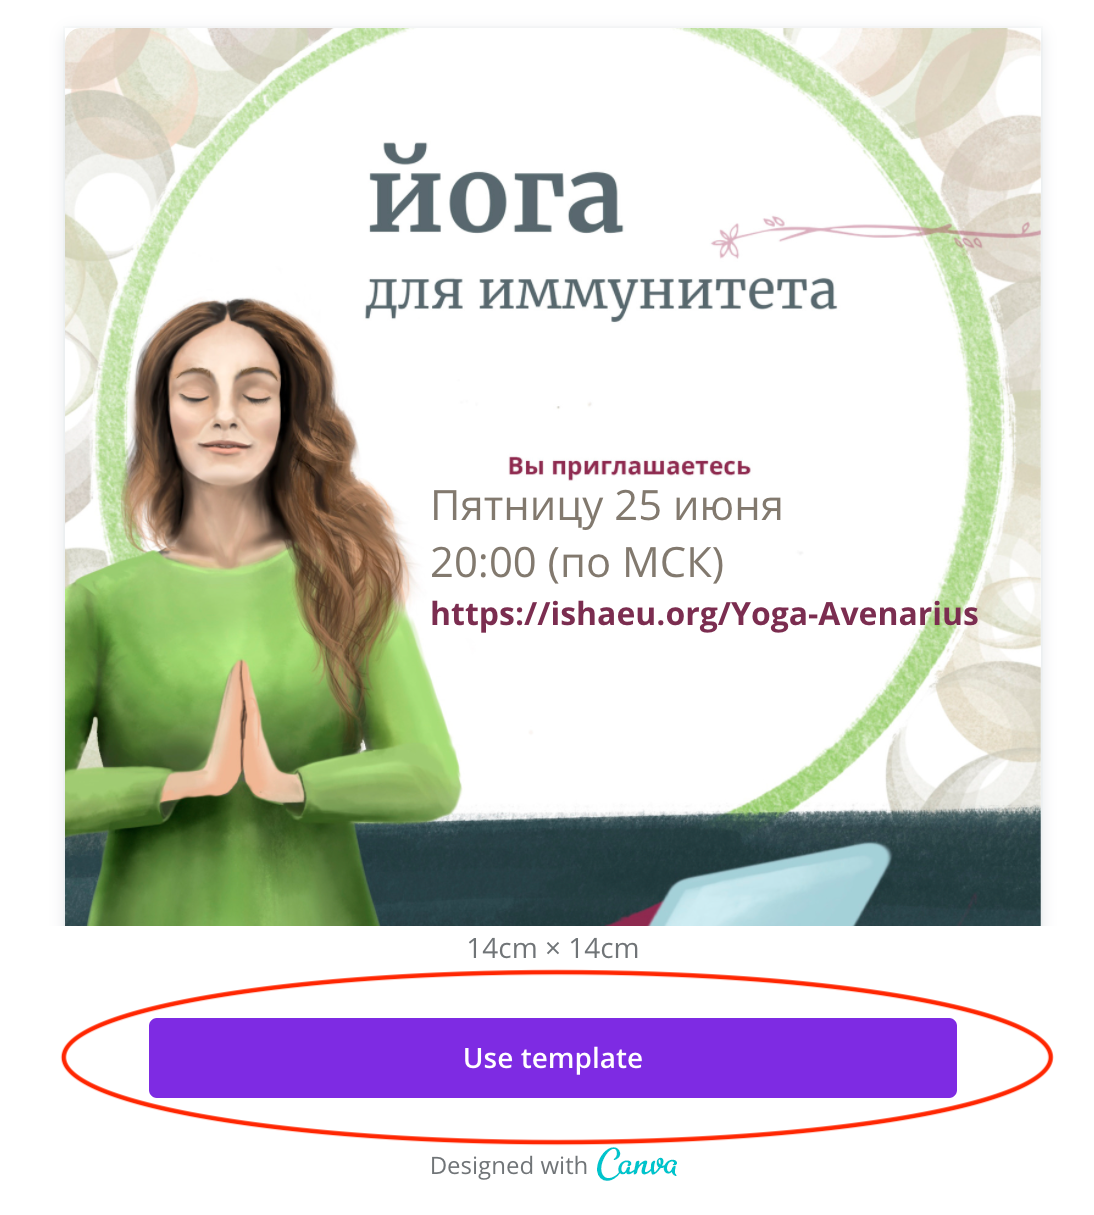
\includegraphics[width=0.59\textwidth]{1canva}
\end{center}

\subsection*{Шаг 2 (изменение)}

Внесите необходимые изменения в тексте изображения. 

\textbf{Мы предоставим вам вашу личную ссылку, используйте ее.}
\begin{center}
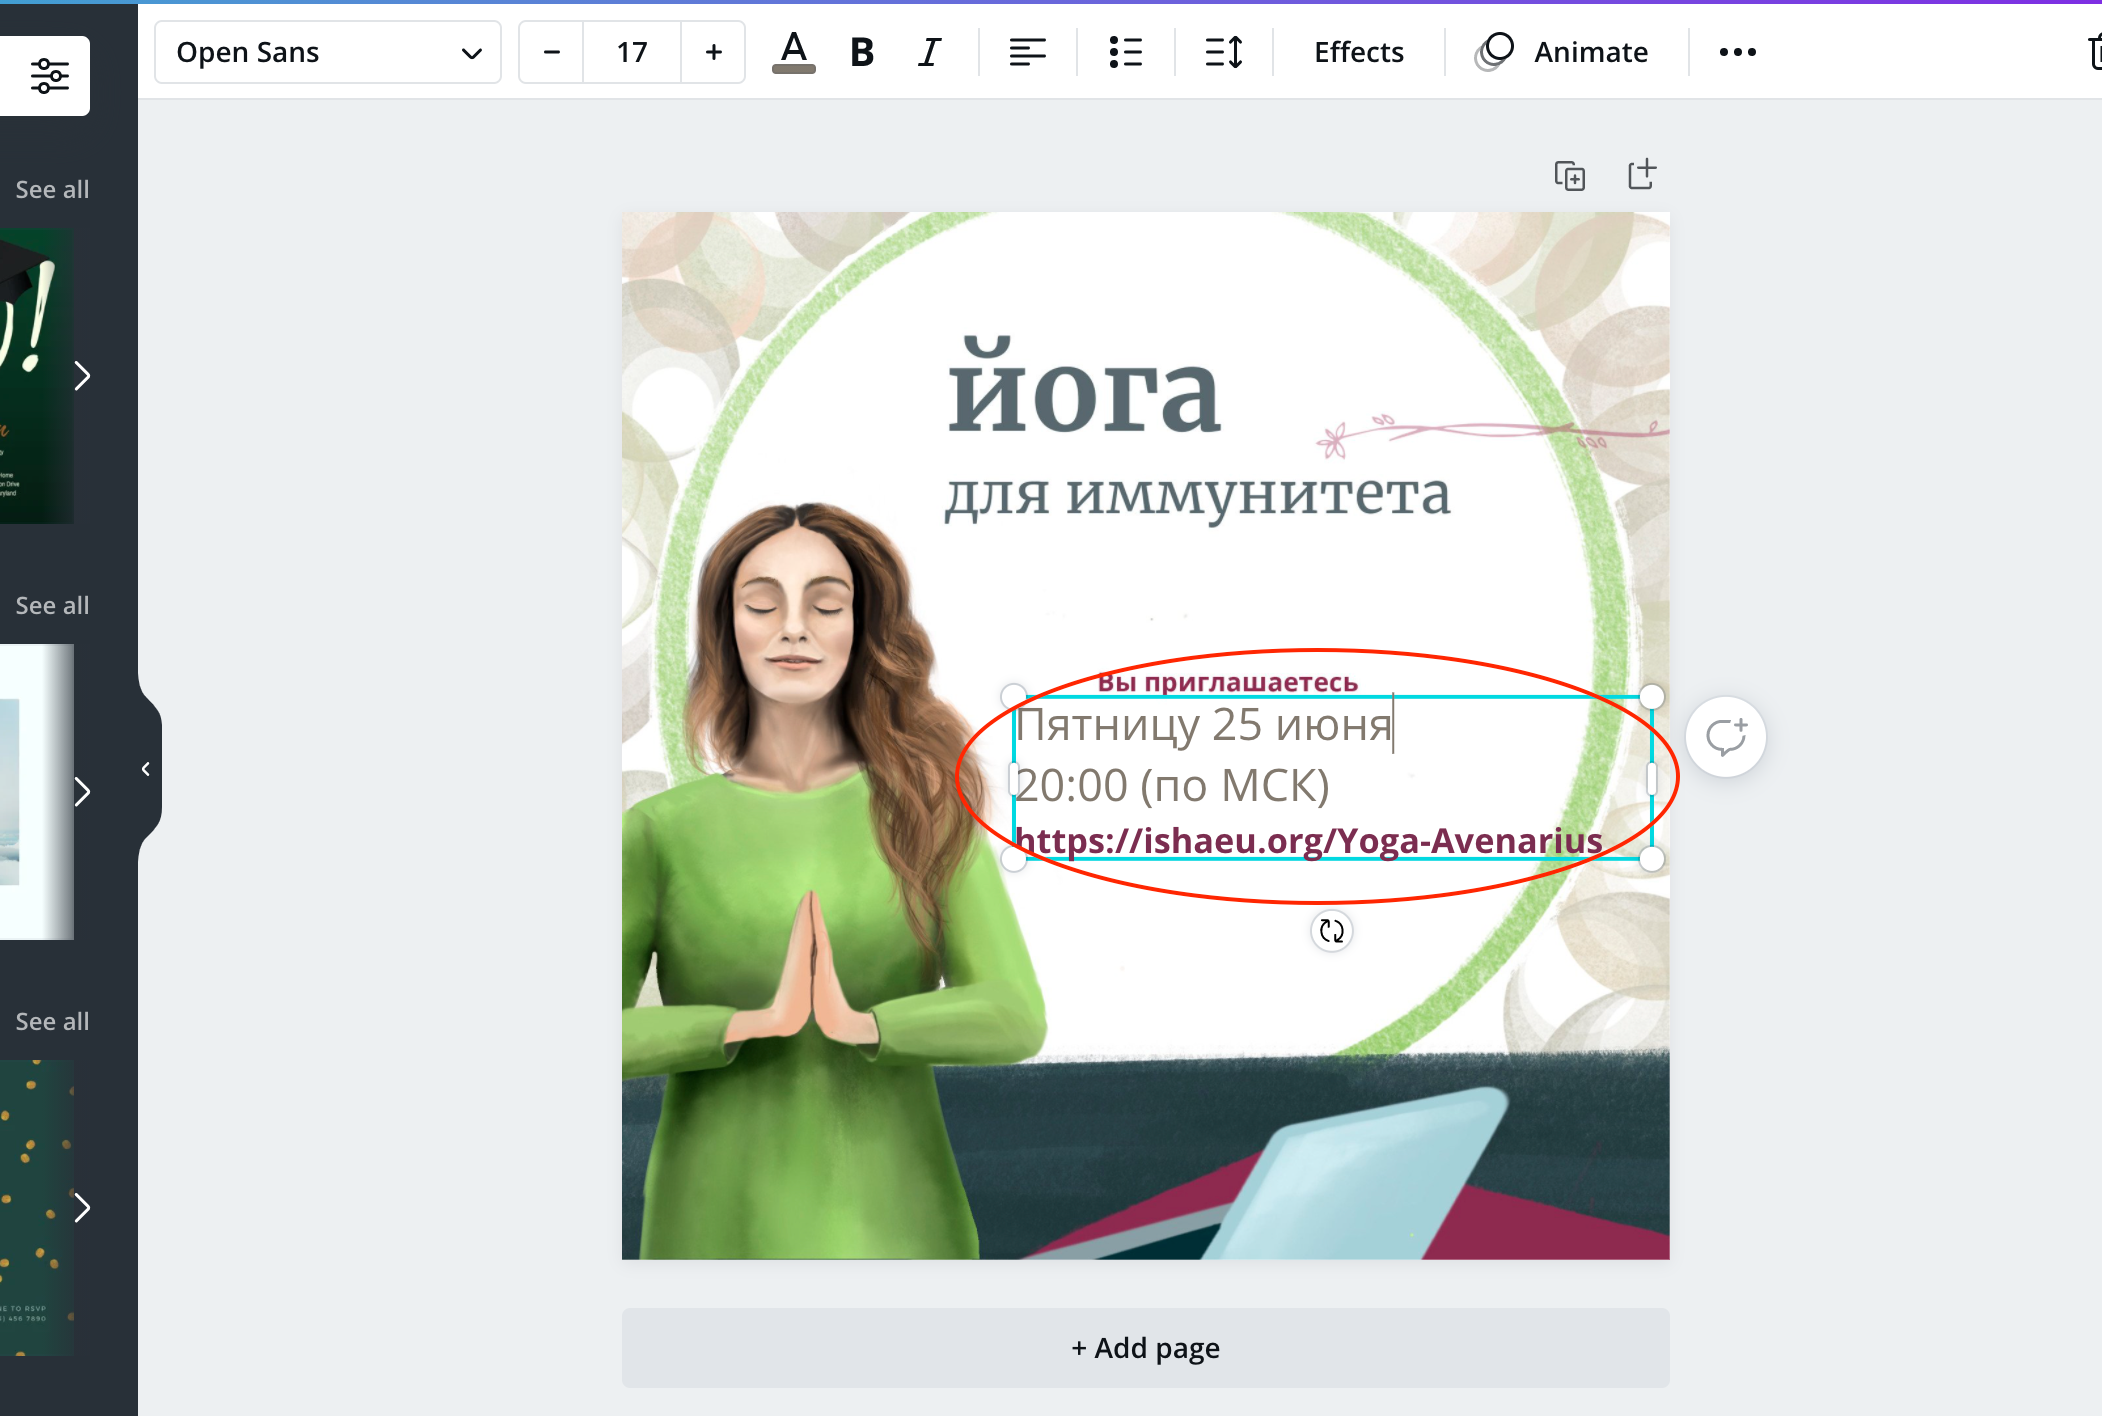
\includegraphics[width=0.59\textwidth]{2canva}
\end{center}
% 
% \subsection*{Шаг 2a (загрузка, если требуется)}
% \begin{enumerate}
% \item Загрузите нужное изображение в Canva. 
% \item Перетащите нужное изображение в поле для дизайна и внесите необходимые изменения. 
% \end{enumerate}
% 


\subsection*{Шаг 3 (экспорт)}
Кликните на кнопку Скачать — Выберите нужный формат изображения: JPEG, PDF и т.д.

Рекомнендуем использовать JPEG, поскольку картинка получается небольшого размера (имеется ввиду размер в байтах).
\begin{center}
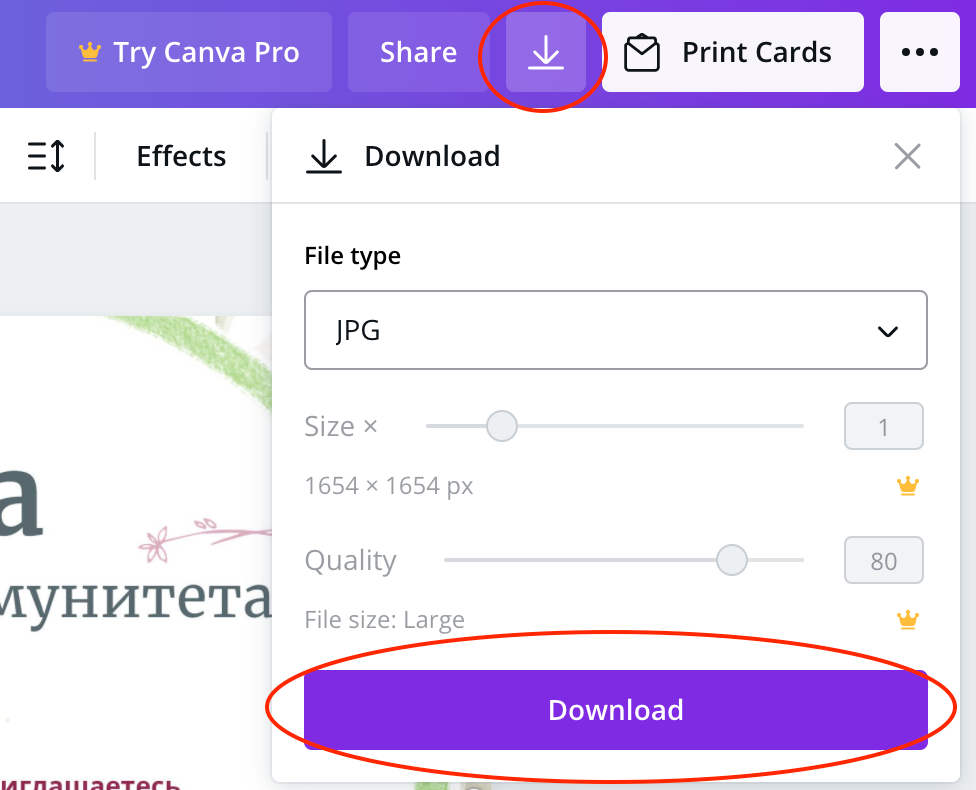
\includegraphics[width=0.59\textwidth]{3canva}
\end{center}


\subsection*{Шаг 4 (радостное использование)}
Откройте скачанное изображение и используйте его для продвижения своих сессий.


